% instead of \usepackage, tikzposter uses this (place before documentclass)
\PassOptionsToPackage{usenames,dvipsnames,svgnames,table}{xcolor}

\documentclass{tikzposter}
\usetheme{Simple}
%\usecolorstyle[colorPalette=BlueGrayOrange]{Default}
\usebackgroundstyle{Empty}

\colorlet{titlebgcolor}{MidnightBlue}
\title{Geometric Partial Matching}
\author{\large Pankaj K. Agarwal, Hsien-Chih Chang, Allen Xiao}

\usepackage[backend=bibtex]{biblatex}
\addbibresource{ref.bib}

\graphicspath{{fig/}}

\def\EMPH#1{\textcolor{MidnightBlue}{\bf #1}}

\def\polylog{\mathop{\mathrm{polylog}}}
\def\eps{\varepsilon}
\def\A{\textcolor{BrickRed}{A}}
\def\B{\textcolor{NavyBlue}{B}}


\begin{document}
\maketitle

\begin{columns}

\column{0.5}
\block{Problem Statement}{
	\EMPH{Geometric Bipartite Matching}:
	Given two equal-sized point sets $\A, \B$ in the plane,
	find a \emph{perfect matching} minimizing the sum of lengths of matching edges.

	\begin{tikzfigure}
	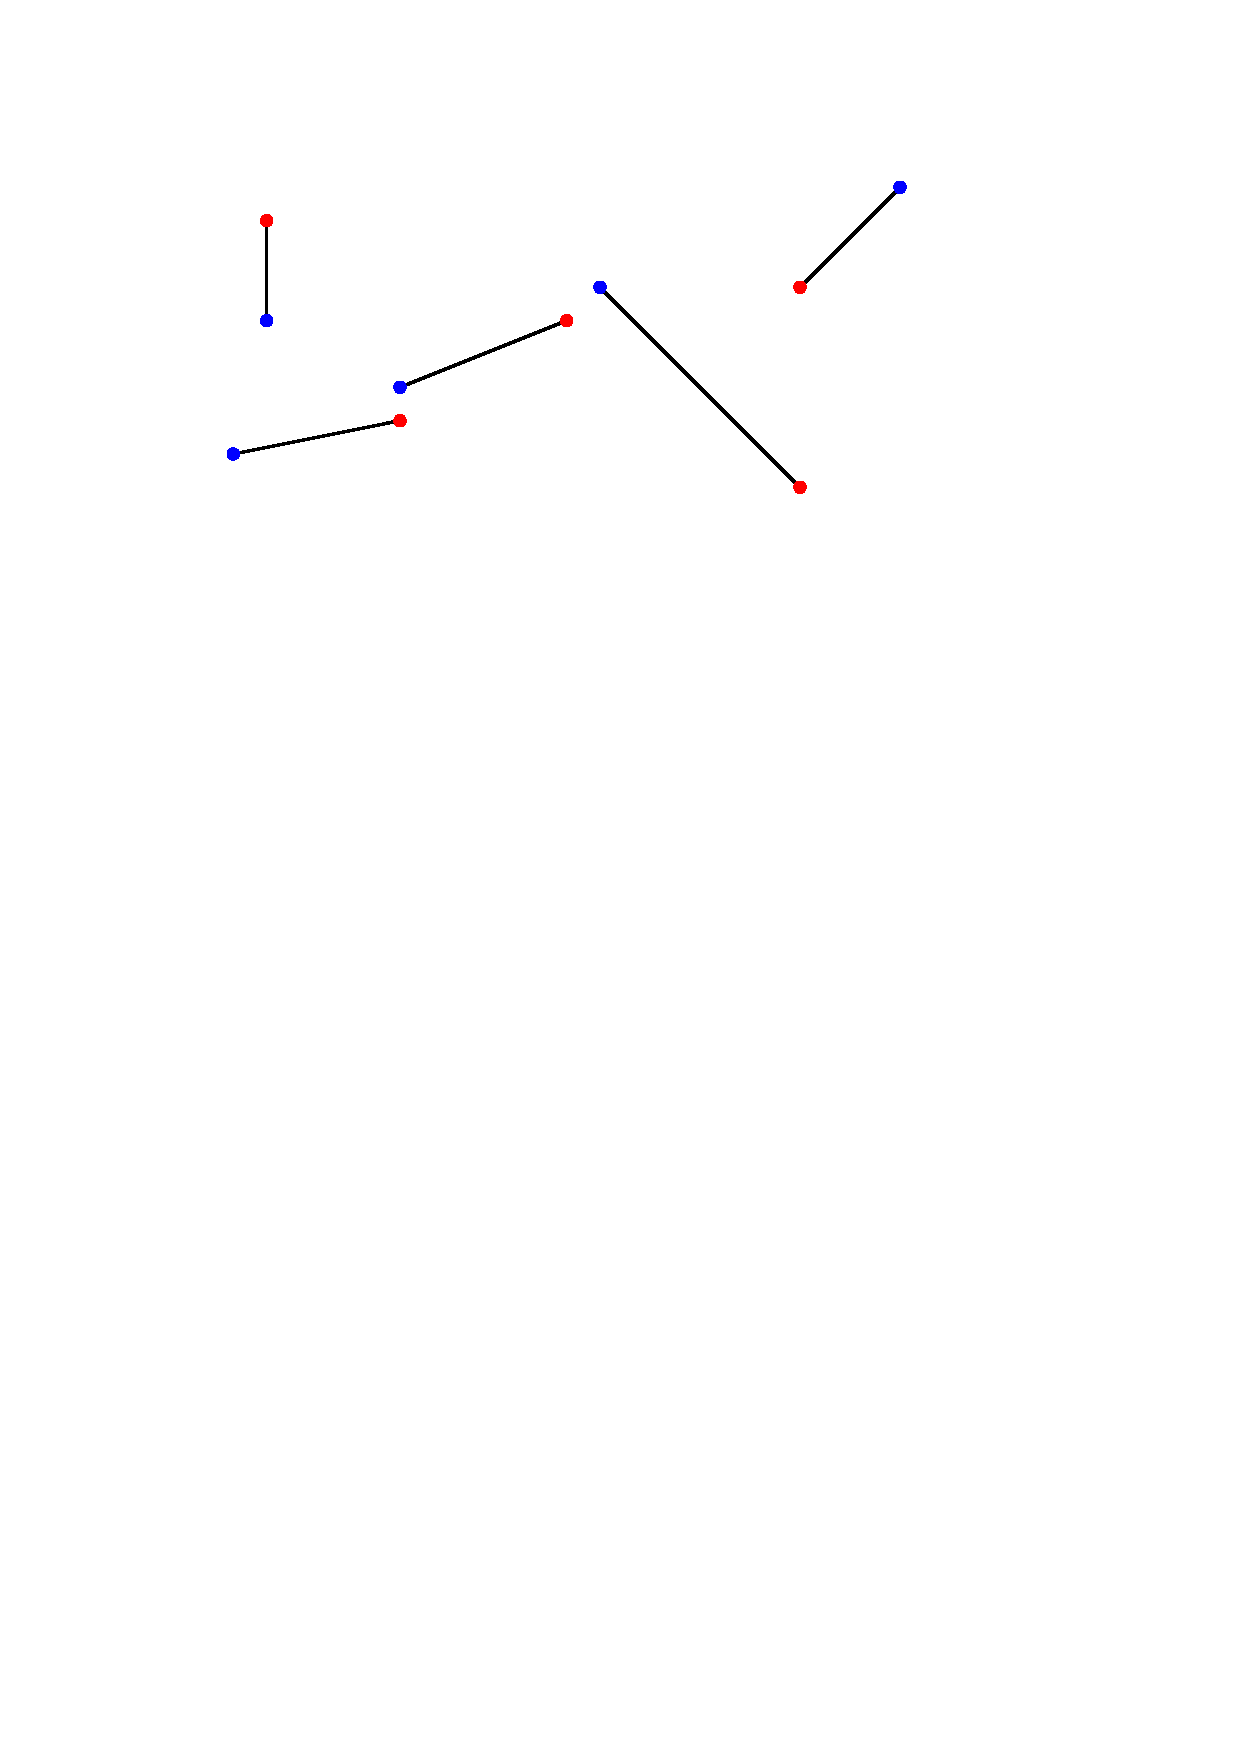
\includegraphics[width=0.9\linewidth,page=1]{matching_vs_partial}
	\end{tikzfigure} 

	\EMPH{Geometric Partial Matching}:
	Given two point sets $\A, \B$ in the plane,
	find a \emph{size-$k$ matching} minimizing the sum of lengths of matching edges.
	(Below, $k = 3$.)

	\begin{tikzfigure}
	\includegraphics[width=0.9\linewidth,page=2]{matching_vs_partial}
	\end{tikzfigure} 

}
\block{Background}{
	Let $n = \max(|\A|, |\B|)$ and $m = |\A \times \B| = O(n^2)$.
	Primal-dual algorithms for general graphs can solve the problem in
	$O(km + k^2 \log n) = O(kn^2 + k^2 \log n)$ time \cite{RT12}.

	However, there are faster algorithms for geometric bipartite matching
	versus perfect matching in general graphs, using dynamic data structures
	for \EMPH{bichromatic closest pair} and \EMPH{nearest neighbors},
	which query/update in $O(\polylog n)$ time \cite{KMRSS17}.
	Roughly speaking, we can replace the $O(m)$ with $O(n\polylog n)$ or
	$O(k\polylog n)$ in many instances.
	If $O(m)$ is no longer the running time bottleneck, can we design a
	faster algorithm for partial matching?
}
\block{Results}{
	Building from existing primal-dual augmentation algorithms:
	\begin{enumerate}
	\item An exact algorithm running in time $O((n + k^2)\polylog n)$,
		using the Hungarian algorithm~\cite{Kuhn55}.
	\item A $(1+\eps)$-approximation algorithm running in time
		$O((n + k\sqrt{k})\polylog n \log(1/\eps))$,
		using a \EMPH{cost-scaling} algorithm for unit-capacity minimum-cost flow
		by Goldberg, Hed, Kaplan, and Tarjan~\cite{GHKT17}.
	\end{enumerate}

	Think of these running times as $O((n + f(k) \cdot k)\polylog n)$ (modulo scaling):

	``After $O(n\polylog n)$ preprocessing time,
	find $f(k)$ augmenting paths in $O(k\polylog n)$ time each.''
}

\column{0.5}
\block{Primal-Dual Augmentation Algorithms}{

	\begin{tikzfigure}
	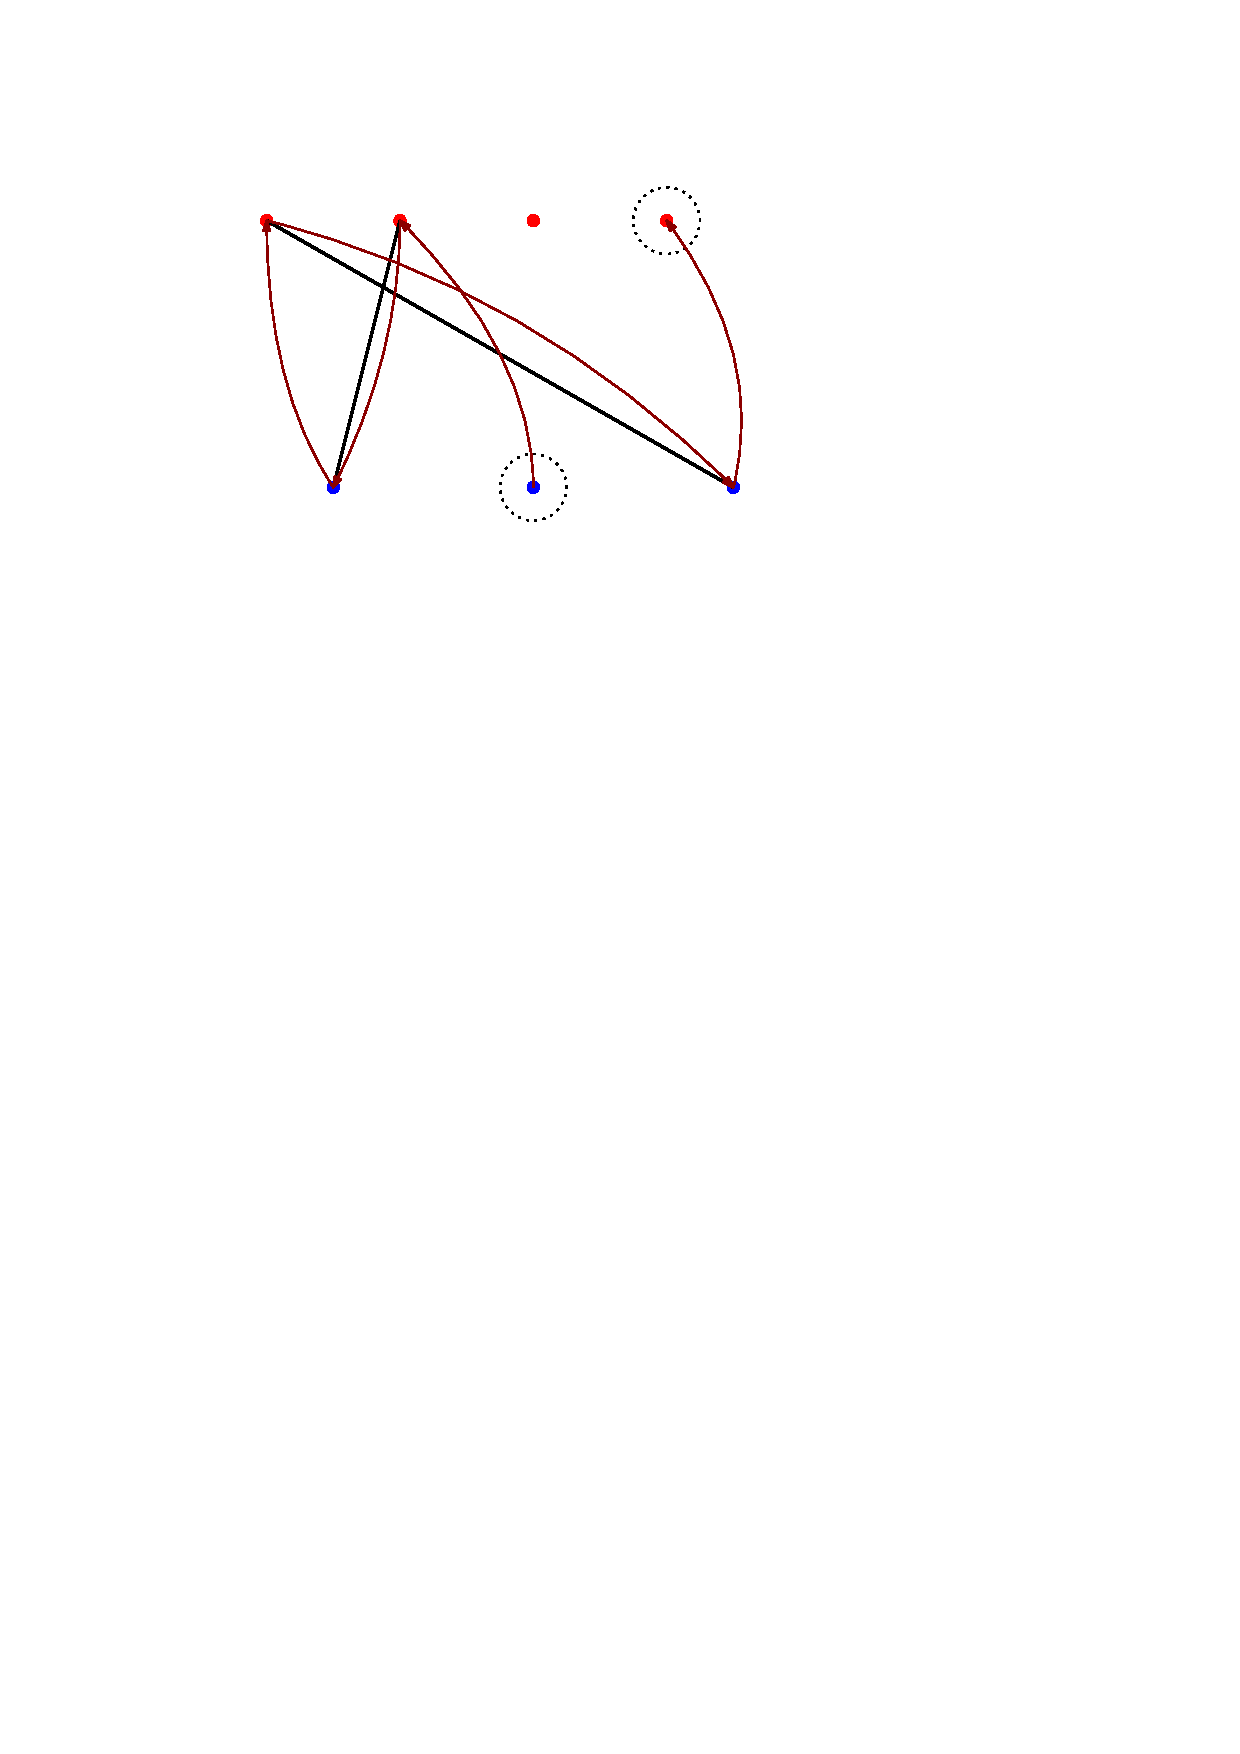
\includegraphics[width=0.9\linewidth]{aug_path}
	\end{tikzfigure} 

	A classical algorithm for min-cost matching and min-cost flow:
	grow the matching using the least-cost augmenting path.
	Essentially, solve a \EMPH{single-source shortest paths} problem (Dijkstra).
	Improves with geometry --- can query the ``next shortest edge'' as a
	bichromatic closest pair for $\A, \B$ in the plane.
}
\block{Our Techniques}{
	% rewinding --- can't reconstruct data structures from scratch; build from the initial state of last iteration
	% skipping dead vertices --- certain vertices cannot be part of an augmenting path, what's left is size O(k)
	\begin{enumerate}
	\item \EMPH{Null vertices}:
		Certain vertices cannot be part of any augmenting path.
		After filtering these out, each BCP query ``makes progress''
		towards finding an augmenting path so the search for an
		augmenting path takes $O(k\polylog n)$ time rather than $O(n\polylog n)$.
		We identify these in our reduction to unit-capacity min-cost flow.

		\begin{tikzfigure}
		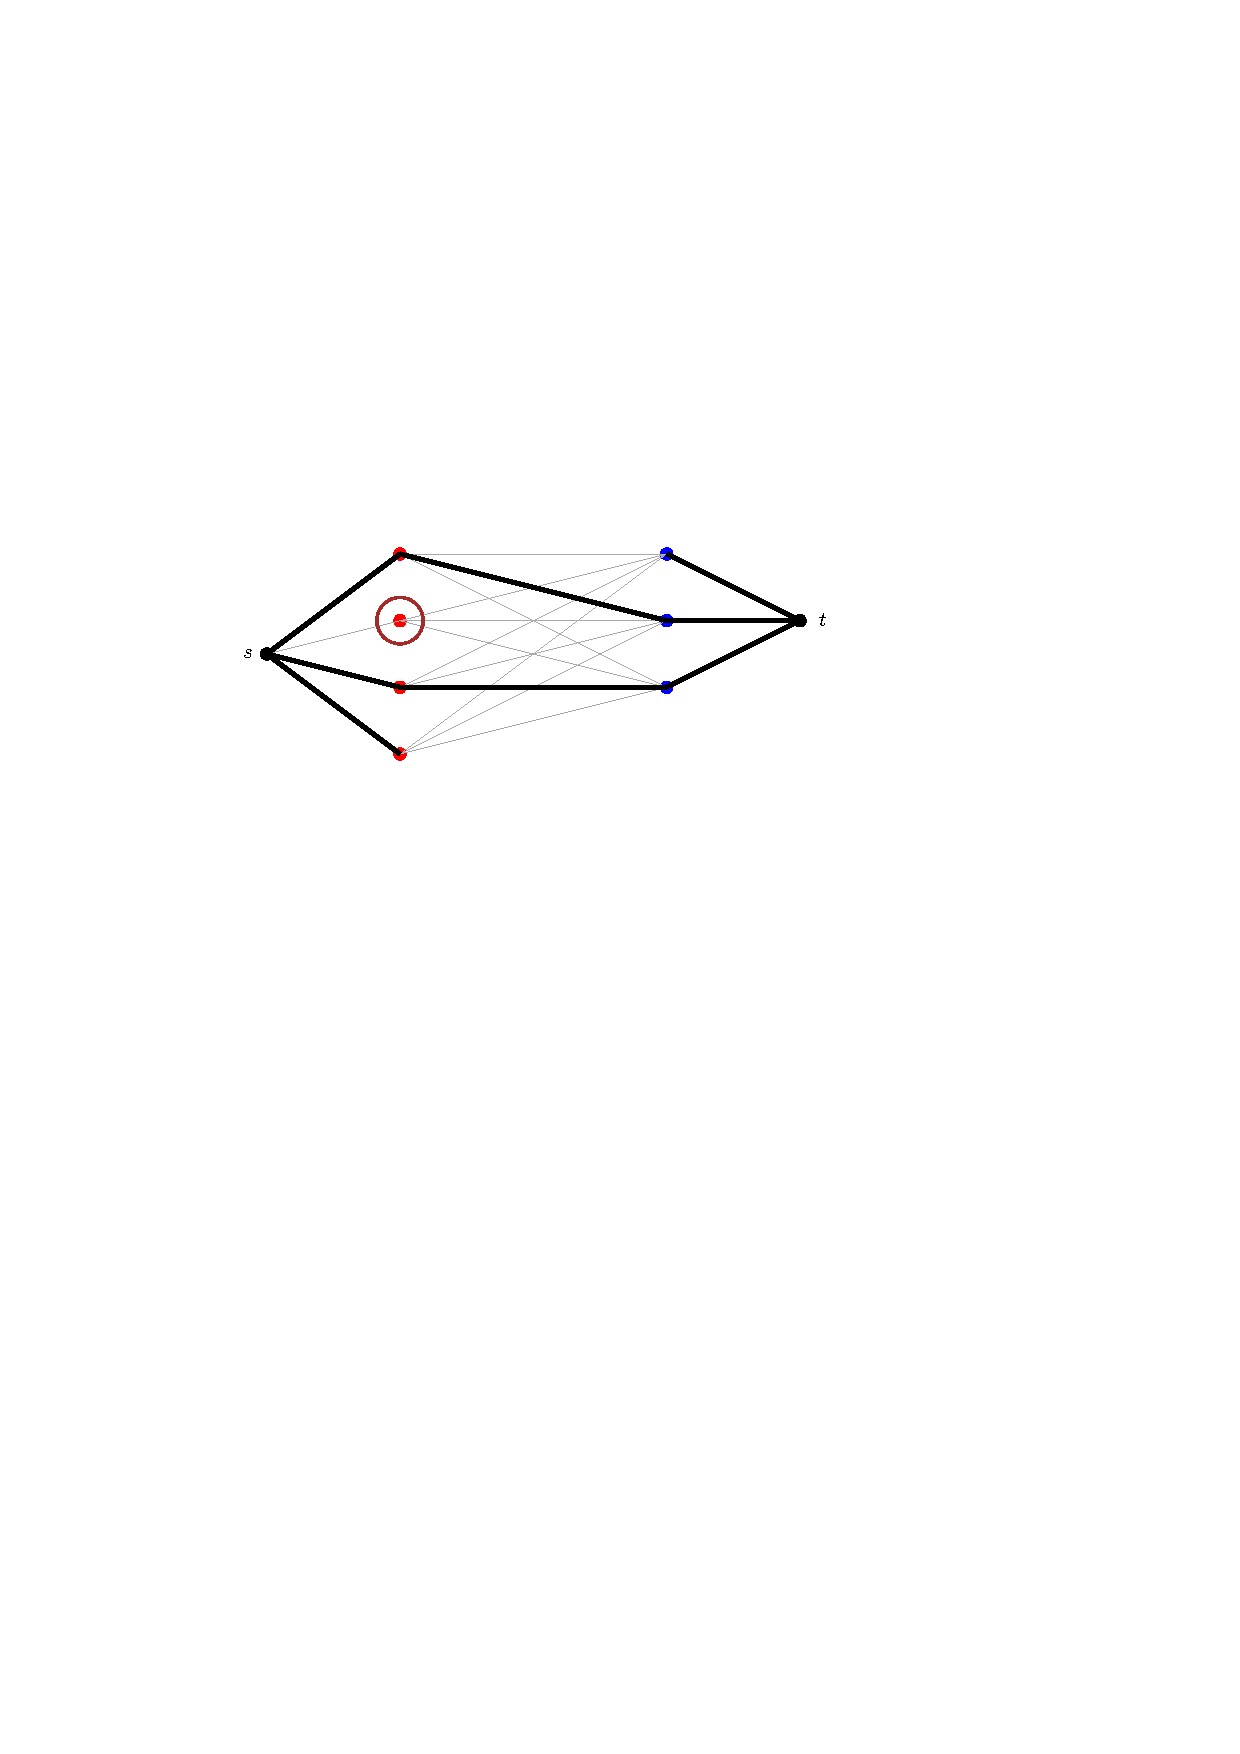
\includegraphics[width=0.7\linewidth]{null}
		\end{tikzfigure} 
	\item \EMPH{Rewinding}:
		It takes $O(n\polylog n)$ time to construct the dynamic data
		structures from scratch.
		We can't afford to do this every augmentation, but we can build
		it from the \emph{initial data structure of the previous
		augmentation} in a single update.
		It costs $O(k\polylog n)$ time to ``rewind'' changes and
		recover the initial data structure state.

		\begin{tikzfigure}
		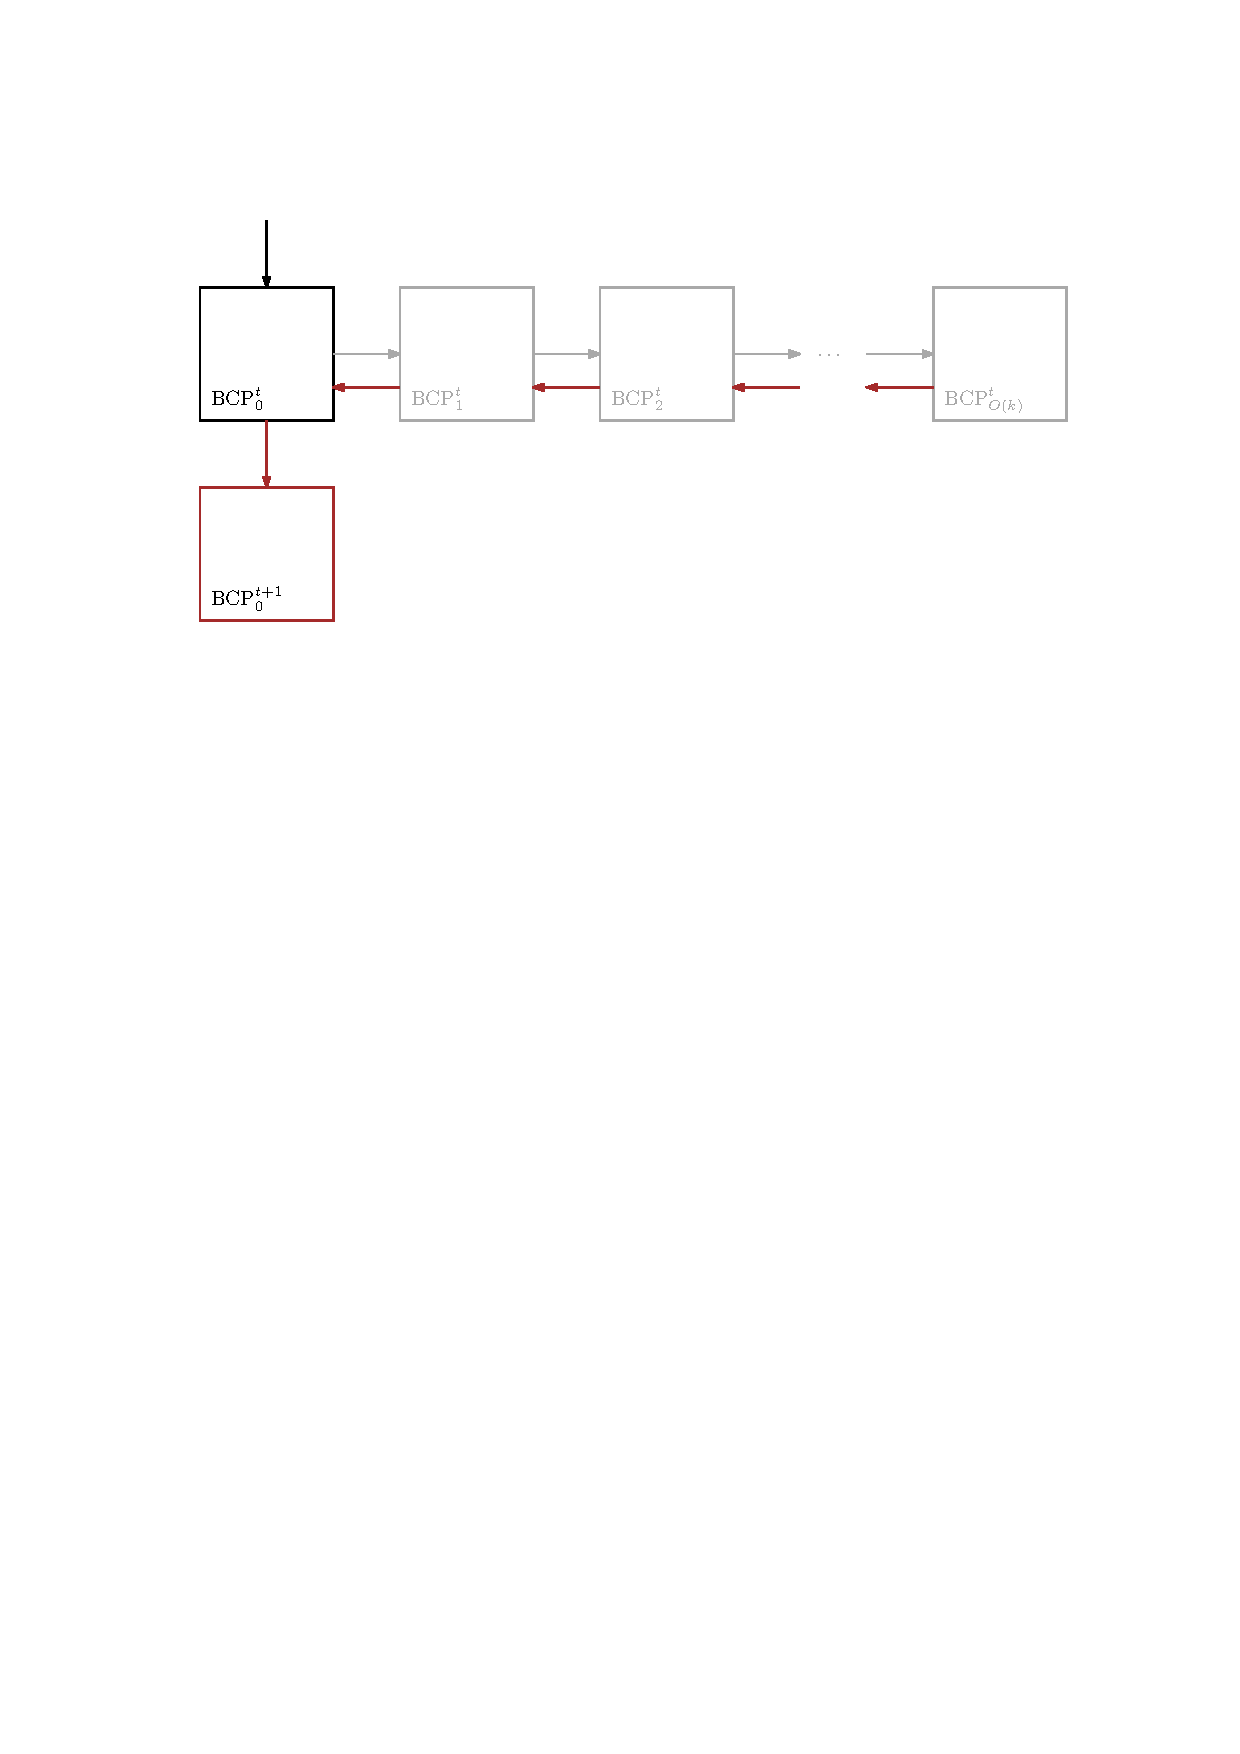
\includegraphics[width=0.7\linewidth]{rewind}
		\end{tikzfigure} 
	\end{enumerate}
}
\block{References}{
	\printbibliography[heading=none]
}

\end{columns}
\end{document}
